\documentclass[conference]{IEEEtran}
\usepackage{amssymb}
\usepackage{graphicx}
\hyphenation{op-tical net-works semi-conduc-tor}

\begin{document}
\title{EEL6935 Course Project Proposal \\
    Sentence Classification Using a CNN}
\author{\IEEEauthorblockN{
    Caleb Bryant\IEEEauthorrefmark{1},
    Jixin Feng\IEEEauthorrefmark{2},
    and Hao Huang\IEEEauthorrefmark{1}}
\IEEEauthorblockA{Department of \\
    \IEEEauthorrefmark{1} Computer \& Information Science \& Engineering\\
    \IEEEauthorrefmark{2} Electrical \& Computer Engineering\\
    University of Florida,
    Gainesville, FL, 32611\\
    Email: \texttt{{\small\{cal2u,fengjixin,haohuang\}}@ufl.edu}}}

\maketitle

\begin{abstract}
    The volume of text on the internet -- unstructured text especially --
    is increasing with drastic speed everyday. Unlike
    human brains, traditional computer programs lack the ability of extracting
    useful information from unstructured text with satisfactory precision.
    While traditional machine learning programs have had limited success
    on NLP problems based on "bag of words" models and feature engineering,
    deep learning and the development of word embeddings have shown
    promising results without the need for feature engineering. In this paper,
    we propose to implement a sentence classification program based on
    convolutional neural networks (CNN) as our course project for
    EEL6935 Big Data Ecosystems.
\end{abstract}

\IEEEpeerreviewmaketitle

\section{Introduction}
    With the tremendous volume of unstructured text generated everyday, on or off
    internet, the demands for processing and extracting useful information
    from it has been constantly increasing. It is predicted that by 2020 the
    total data volume of ``digital universe'' will increase to 40 ZB
    ($40\times 10^{21}$ bytes), which is about 50 times more than the size of
    year 2010\cite{gantz2012digital}. Most of the text will be generated by various
    sources like news media, social networks, medical records, etc.

    Although this text data is a valuable source of information
    and can be easily comprehended by humans, current computational methods
    continue to struggle extracting information from unstructured text sources\cite{mitchell2015}.
    Hence effective methods to process and analyze unstructured text data are
    desperately needed.

    In this course project, we are targeting a specific domain of text analysis
    problems -- sentence classification. The goal of sentence classification is to assign
    proper pre-defined labels to a given sentence, so that the main subject of the
    sentence can be represented and then categorized\cite{allahyari2017brief}.
    Mathematically, the classification model can be represented as:
    $$f:\mathcal{D}\rightarrow\mathcal{L}$$
    where $\mathcal{D}=\{d_0, d_1,\ldots, d_{n-1}\}$ is the set of sentences
    (sentence), and $\mathcal{L}=\{l_0, l_1,\ldots, l_{k-1}\}$ is the set of labels.
    Depending on whether multiple labels are allowed to assigned to a document, the
    classification is called soft or hard\cite{gopal2010multilabel}.

    The performance of a sentence classification system can be evaluated with its
    F-1 score, which can be defined as\cite{forman2003extensive}:
    $$F_1=\frac{2}{\frac{1}{r}+\frac{1}{p}}=\frac{2pr}{p+r}$$
    where $p=\frac{tpr}{tpr+fpr}$ stands for precision and $r=\frac{tpr}{tpr+fnr}$
    stands for recall.

    Historically, sentence classification has been done via statistical
    and machine learning methods like Naive Bayes, k-nearest neighbors, decision
    trees, SVM, etc. In this proposal, we decide to implement sentence classifier
    using a convolutional neural network (CNN), a deep learning model. By definition
    CNN uses multiple layers of convolving filters that apply on the input data and
    calculate the output after all feeding the input through all of the layers. Although
    originally built for computer vision, CNNs have shown quite significant potential in
    natural language processing (NLP), and especially in sentence classification.
    \cite{kim2014convolutional}.

\section{Proposed System Model}
     Our chosen network architecture is based upon Yoon Kim's work on sentence
     classification\cite{kim2014convolutional}. The architecture consists of four main parts: a word
     embedding layer, a convolution layer, a pooling layer and a fully connected layer
     at the end.
    \begin{figure*}
    \center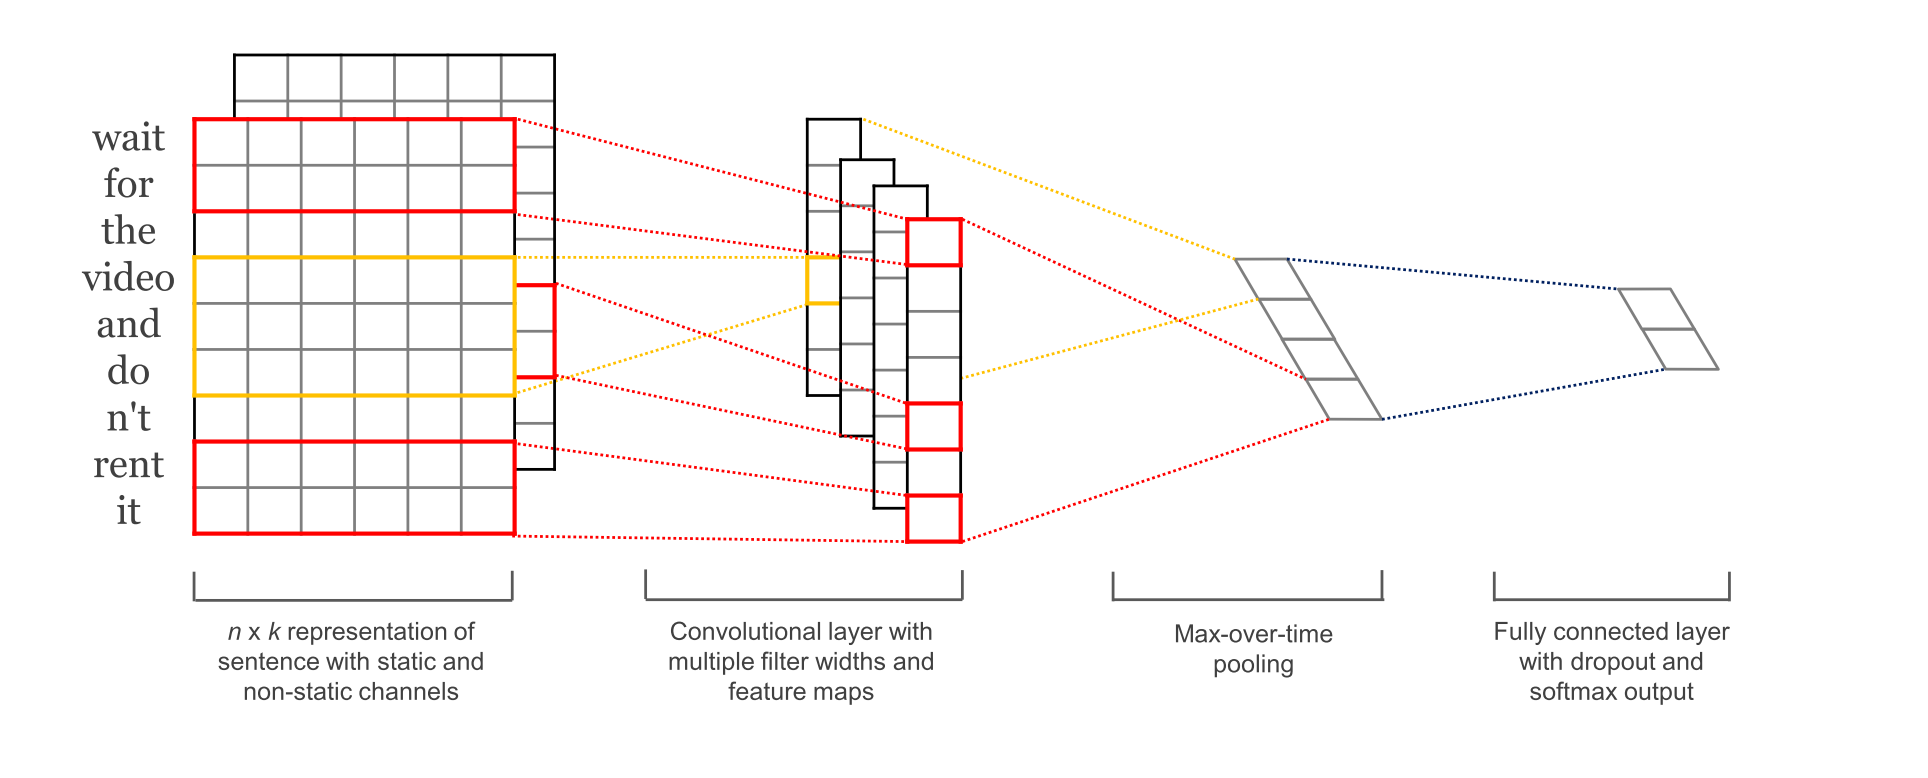
\includegraphics[width=0.9\textwidth]{figure/sc_model}
    \caption{Model architecture with two channels for an example sentence,
        figure credit: \cite{kim2014convolutional}}
    \end{figure*}

     Distributed word embeddings, which were popularized by Mikolov et al.
     in 2013\cite{word2vec}, allow us to represent a word as a vector in
     multi-dimensional space, and they form the basis for feeding text into our deep
     learning model.

     Let $x_{i} \in \mathbb{R}^k$ be a dimentional word vector representing the $i$-th word in the
     sentence. Thus, the sentence would be represented by
     \begin{equation}
      x_{1:n} = x_1 \oplus x_2 \oplus ... \oplus x_n
      \end{equation}
      Where $\oplus$ signifies concatenation. Suppose $x_{i:i+j}$ refers to concatenating
      word vectors $x_i, x_{i+1}, ... , x_{i+j}$. The convolution operator with a filter
       $W \in \mathbb{R}^{hk}$ applied to a window size of $h$
      words is defined as
      \begin{equation}
      c_i = f(W \cdot x_{i:i_{h-1}} + b)
      \end{equation}
      Where $b$ is a bias term and $f$ signifies a non linear function such as the hyperbolic
      tangent. We use this filter to generate a feature map $c = [c_1, c_2, ... ,x_{n-h+1}]$
      with $c \in \mathbb{R}^{n-h+1}$ by applying the filter to each possible window of words in
      the sentence $x_{1:h}, x_{2:h+1}, ... ,x_{n-h+1:n}$.

      We plan to use multiple filters with varying window sizes to obtain multiple features, and we will
      compare our results for different hyperparameters.
      A max-over-time pooling operation $\hat{c}$ = max\{$c$\} will be applied once the feature
      maps are generated. The pooling operation outputs the largest value from each individual
      feature maps. We will employ dropout on the penultimate layer $z = [\hat{c}_1,...,\hat{c}_m]$
      (we have $m$ filters) for regularization with a constraint on $l_2$-norms of the weight
      vectors. This should help prevent co-adaptation of hidden units by randomly setting weights
      to zero for selected neurons. The function is expressed below:

      \begin{equation}
       y = W \cdot (z \circ r) + b
      \end{equation}

      where $\circ$ is the element-wise multiplication operator and $r \in \mathbb{R}^m$ is
      the masking vector of Bernoulli random variables with probability $p$ of being 1.
      The gradients are backpropagated through the unmasked units during training. At test
      time, the learned weight vectors are scaled by $p$ such that $\hat{w} = pw$ and $\hat{w}$
      is used to score unseen sentences. Finally, we will constrain $l_2$-norms of the weight
      vectors by rescaling $w$ to have $||w||_2 = s$ whenever $||w||_2 > s$ after a gradient
      decent step.

\section{Proposed Simulation Scenarios}
      To test and evaluate our model, we propose using the Stanford Large Movie Review
      Dataset to preform sentiment classification\cite{maas-EtAl:2011:ACL-HLT2011}.
      The dataset contains 50,000 highly polar
      movie reviews, and we will score each movie review as either positive or
      negative. We will use a 60/20/20 split for training, development, and testing.

      In addition to using the above data set, we will also train and test using the Stanford Sentiment
      Treebank, which is one of the data sets Kim evaluated in his paper\cite{sentimenttreebank}.
      Using the same data set
      will allow us to compare our model with Kim's model directly. Both binary (positive/negative)
      and fine-grained (scale from 1-5) classification tasks will be performed and scored for accuracy.
      For all tasks, we will compute the accuracy of our model by diving the number of correct classifications
      by the total number of test samples.

      We will be implementing the model using Python and Tensorflow. The simulations will be conducted on
      computers with a 3.1GHz Intel Core i7 CPU with 8MB cache and 16GB RAM running Ubuntu 14.04 LTS.

\section{Conclusion}
In this proposal we presented a convolutional neural network based on Kim's paper for sentiment
analysis on a number of data sets. We have also proposed a test plan to evaluate the performance of our
deep learning architecture.

\bibliographystyle{IEEEtran}
\bibliography{eel6935_proposal}

\end{document}
